\chapter{Literature Review}

\textsl{The purpose of the current chapter is to provide knowledge of the subject areas relevant to the project including current developments, controversies, breakthrough, previous research and relevant background theory.}


\section{Market Research Systems}
\ac{MRS}s use big data analytics and online methods to produce high quality marketing information that medium sized companies can use to understand their market and be more competitive \cite{digitaltrasformationsmes}. Marketing research is useful in the area of product planning and development such as when evaluating the need for a new product or its positioning in the market. It has applications in the area of advertising and copy testing or to identify existing and potential distribution channels. It can help to deduce the pricing expectations of consumers and their reactions and responses to different price levels of products. Marketing research can identify the forces operating in a market and assess the market trends, the size of present and potential markets of the company, the evolution of the impact of government legislation, policies, and schemes on the performances of marketing operations of the company. It can also study the sales potential of the company’s products and the evolution of the company’s sales performance. Finally, it can assess the environmental fitness of the firm. \cite{marketingresearch}. A study conducted by the Alibaba Group in China has also shown a way of calculating the impact of brands on society, by combining the impact brands have on the media, the government Impact and the personal impact. \cite{brandsimpact} The \ac{MRS} can obtain all these analytics by integrating several data sources and where necessary apply AI and Machine learning to deduce useful results \cite{marketingml}. Platforms like QuantCloud, a trading service \cite{quantcloud}, or Google Analytics, a websites activity tracking platform \cite{googleanalytics}, all offer insights within specific areas and require specialized knowledge to be used. The goal is to build a prototype of a \ac{MRS} that generates a variety of marketing information automatically and that does not require specialized knowledge.



\section{AI, ML and Big Data}
Big data is a term used to describe the huge amount of data that is being generated by organizations in today’s business environment. Such data usually comes from three primary sources: social data such as likes, tweets, comments, video uploads, queries in search engines etc., machine data generated by sensors installed in industrial equipment and transaction data. Machine learning is a branch of artificial intelligence that provides tools and techniques for working on all this data to produce useful results. It is based on the idea that systems can learn from data, identify patterns and make decisions with minimal human intervention. Machine learning algorithms are classified into supervised learning, unsupervised learning and reinforcement learning \cite{marketingml}: 

\subsection{Supervised learning}

Supervised learning is the task of training a function with labelled training data in order for this function to be able to learn a general rule and map any input to its appropriate output. Machine learning models are usually very good at performing regression and classification:

\begin{itemize} 
	\item Statistical modelling techniques are used to find a parametric function that best fits a set of observations and train it appropriately so that is can predict new observations. Statistical models (i.e. logistic models, polynomials, linear regression models) are very good at modelling and predicting trends;
	\item Neural networks are powerful tools used to perform regression and classification of non linearly separable data. For example, convolutional neural networks can be used to classify consumers according to their preferences so that they can be targeted by specific ads or marketing strategies \cite{socialtrends}. Neural Networks, paired with Locality sensitive hashing \cite{lsh} can be used to improve de-duplication, that is to identify chunks that are already stored in a large database;
	\item Kernel Machines can perform accurate regression and classification by mapping the data feature space into an equivalent higher order representation where the problem becomes linearly separable. They are very good at analysing non stationary data such as marketing trends \cite{onlineregressionkernels};
	\item Support Vector Machines are excellent regression and classification algorithms that work by separating the data set with an hyperplane and maximizing the margin between the closest points. They can be employed to classify social media data such as tweets, posts, comments etc. according to the emotions they emit (positive, negative and neutral). These results can aid in understanding if people have a good or bad opinion about something and take action accordingly \cite{sentimentanalysis}.
\end{itemize}  


\subsection{Unsupervised learning}
Unsupervised learning is a machine learning technique in which a model works on its own to discover hidden patterns and separate unlabelled information into appropriate clusters, if they exist. It is useful for finding associations between different parameters in the available data, for example people that buy X might also buy Y. It can also be used to find the anomalous elements in a data set \cite{kmeans}. There exist several clustering methods:
\begin{itemize} 
	\item Hierarchical clustering is a naive clustering method that builds a hierarchy of clusters by iteratively joining together the closest elements;
	\item K-means is a set of unsupervised clustering algorithms that can divide data points into k clusters  \cite{kmeans};
	\item K-Nearest Neighbors is an algorithm that finds the k nearest points to the point of interest.
\end{itemize}

\subsection{Reinforcement learning}
Reinforcement learning is the training of machine learning models to make a sequence of decisions. The agent learns to achieve a goal in an uncertain, potentially complex environment \cite{reinforcementlearning}.
\begin{itemize} 
	\item Monte Carlo methods are a way of obtaining estimates when working with uncertain phenomena. They use randomness to obtain meaningful information and are effective for calculating business risks and predicting costs or scheduling overruns;
	\item For any finite Markov decision process, Q-learning algorithms are able to find an optimal path by maximizing the expected value of the total reward over any and all successive steps, starting from a specific state. These algorithms can be used to make decisions in business environments, for example in order to determine whether to hold, buy, or sell at any point in time.
\end{itemize}

\newpage
\section{ML workflow}

\begin{figure}[H]
	\centering
	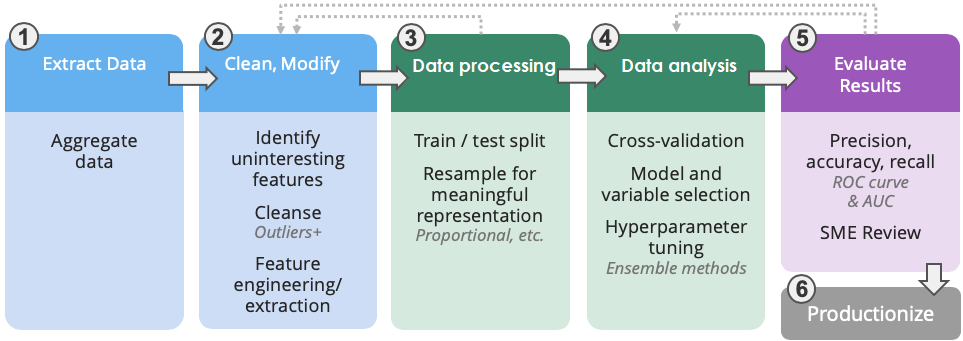
\includegraphics[scale=0.8]{img/mlworkflow.png}
	\caption{A machine learning task includes data gathering/extraction, data cleaning, data processing, data analysis, training and testing and finally the evaluation phase.}
	\label{Literature Review:Machine Learning}
\end{figure} 

A machine learning task typically involves collecting, transforming, cleaning, and modelling data with the goal of discovering new information \cite{mlworkflow}.



\subsection{Data aggregation}
Data aggregation is the process of gathering data and presenting it in a summarized format. The data may be gathered from multiple local or remote data sources with the intent of combining these data sources into a common model that could be virtual. Time aggregation collects data points for a single resource over a specific time frame, while spatial aggregation gathers a time series from a group of resources. It is possible to store incoming data into a Data warehouse, which is a large centralized repository of data.

\subsection{Data cleaning}
Before data can be fed to a training algorithm or used for numerical analysis, it is important to prepare it by removing or changing rows that are incorrect, incomplete, irrelevant, duplicated, or improperly formatted. In some cases it is necessary to map data to another model. Skipping this step is not recommended because it can lead to runtime errors, inaccurate results and false conclusions \cite{quantcloud}. 

\subsection{Data processing}
The data is divided into 3 three different sets, the training set, the validation set and the test set. During this phase some dimensions of the data might be removed, merged together or reshaped depending on the kind of task to be performed. 

\subsection{Data analysis}
 Predictive analytics, artificial intelligence (AI) or machine learning algorithms can be applied to the collected data for new insights. Depending on the task at hand (regression or classification) an array of ML models and sets of optimal hyper parameters are chosen for training. 

\subsection{Evaluation}
The chosen models are trained with the training data and their precision, accuracy and recall are compared in order to find the best model and understand how well the chosen model can work in the future.

\subsection{Deploying to production}
Only the most accurate models are deployed to production. Marketing data display non stationary behaviour and cannot be accurately modelled by statistical models. On the other hand kernel machines are able to model well data that displays dynamic means, variances, and covariances.

\newpage
\section{Kernel recursive least-squares regression methods}
Marketing data is non-stationary which means that it is affected by several implicit variables; some data points might belong to different distributions or they might be affected by seasonal patterns and other external influences. Because of this it is very difficult to model marketing data and perform accurate forecasting. Kernel machines offer a way of modelling such unpredictable data sets. Kernel methods use the kernel trick and adaptive filters such as the Recursive Least Squares (RLS) method to update sample-by-sample a regression model \cite{onlineregressionkernels}. A linear regression model \(f(x)=w^\mathsf{T}x \) with \(x, w \in \mathbb{R}^\mathsf{D}\) and \(y \in \mathbb{R} \) can be  reformulated into a convex optimization problem \(f(x)=\sum_{n=1}^{N} [\alpha(n)\kappa(x_n, x)] \) where \(\alpha(n) \in \mathbb{R} \) are the expansion coefficients and \(x_n\) are the training data or bases. In this reformulation the kernel function \(\kappa(x, x^\mathsf{'})=\phi(x)^\mathsf{T}\phi(x^\mathsf{'}) \) can be interpreted as inner products in a high-dimensional feature space (more formally called Hilbert space), and these can be calculated without having direct knowledge of the higher order feature space. By doing this operation a non linearly separable problem can be brought in a space where it is linearly separable. The least squares minimization \(\frac{\partial J(w)}{\partial w}=0\) yields the coefficients \(\hat{w} = \phi^\mathsf{T}a\), that can be substituted into \(J(w)\) creating the dual representation \(J(a)\). The minimization \(\frac{\partial J(a)}{\partial a} = 0\) yields the coefficients \(\hat{a} = (K + \lambda I_N)^\mathsf{-1}t\), which can be substituted inside the linear regression model to obtain a kernel-based prediction model:
\[f(x)=w^\mathsf{T}\phi(x)=a^\mathsf{T}\phi\phi(x) = k(x)^\mathsf{T}(K + \lambda I_N)^\mathsf{-1}t\]
Because the solution to the least-squares problem is expressed as a linear combination of the training data and in terms of the parameter vector w and the kernel function k, it does not matter how complex the feature vector \(\phi(x)\) is and it can even have infinite dimensionality if that suits the problem at hand. \\

When using this method in an online scenario if a new data point is made available it's possible to update the weights of the model recursively by the previous solution calculated with the last \(n-1\) data points. The updated solution \(\alpha(n)\) is obtained by recursively applying:
\[\alpha(n) = \begin{bmatrix} \alpha(n-1) - \frac{a_n e_n}{\gamma_n} \\ \frac{e_n}{\gamma} \end{bmatrix}\]
where \(e_n = y_n-\hat{y_n}\), \(a_n = K_{n-1}^\mathsf{-1}k_n\) and \(\gamma_n = k_{nn} + c - k_{n}^\mathsf{T}a_n\).\\

The algorithm can be optimized further by using a sliding window that stores the last M data points. When a new data point is made available, before updating the solution, the algorithm adds the new datum to the sliding window and discards the oldest datum or the data point that causes the least error upon being discarded.\\

Finally it's possible to improve accuracy further by using a Gaussian process model \(y = f(x) + r\) which has a zero mean GP prior on f(x) and a Gaussian prior on r. It can be found that the posterior over the latent vector f is \(p(f | y) = \mathcal{N} (f|\mu \Sigma)\) which means that the result of this model gives not only the mean value for the predicted solution but also its entire posterior distribution. The recursive updates of the model are:
\(p(f_{n}|X_{n}, y_{n}) = \mathcal{N} (f_{n}|\mu_{n}, \Sigma_{n})\), \(\mu_{n}= \begin{bmatrix} \mu_{n-1}\\ \hat{y}_{n} \end{bmatrix} + \frac{e_{n}}{\hat{\sigma}^{2}_{y_{n}}}\begin{bmatrix} h_{n}\\ \hat{\sigma}^{2}_{f_{n}} \end{bmatrix}\), 
\( \Sigma_{n} = \begin{bmatrix} \Sigma_{n-1} & h_{n} \\ h_{n}^{T} & \hat{\sigma}^{2}_{f_{n}} \end{bmatrix} - \begin{bmatrix} h_{n}\\ \hat{\sigma}^{2}_{f_{n}} \end{bmatrix} \begin{bmatrix} h_{n}\\ \hat{\sigma}^{2}_{f_{n}} \end{bmatrix}^{T} \), where \(h_n = \Sigma_{n-1}K_{n-1}^{-1} k_{n}\) and \(\hat{\sigma}^{2}_{f_{n}}\) and \(\hat{\sigma}^{2}_{y_{n}}\) are the predictive variances of the latent function and
the new output calculated at the new input. The underlying Gaussian process is described at every point by \( \mu_{n} \) and \( \Sigma_{n} \). The entire KRLS-T algorithm is summarized in algorithm \ref{Literature Review:KRLS-T}. KRLS-T was used in this thesis to implement regression and perform forecasting.

\begin{algorithm}
	\caption{KRLS Tracker (KRLS-T) algorithm.}
	\label{Literature Review:KRLS-T}
	\begin{algorithmic}
		\FOR{$i=1, 2, ...$}
		\STATE FORGET: \(\mu_{n-1} \leftarrow \sqrt{\lambda} \mu_{n-1}\), \(\Sigma_{n-1} \leftarrow \lambda \Sigma + (1 - \lambda) K\).
		\STATE Observe input \(x_{n}\).
		\STATE Calculate predictive mean: \(\hat{y_{n}}=k_{n} K_{n-1}^{-1} \mu_{n-1}\)
		\STATE Calculate predictive variance: \(\hat{\sigma}^{2}_{yn}\).
		\STATE Observe true output: \(y_{n}\)
		Compute \(\mu_{n}\), \(\Sigma_{n}\), \(K_{n}^{-1}\).
		\STATE Add basis \(x_{n}\) to the dictionary.
		\IF{number of bases in the dictionary > M}
		\STATE Determine the least relevant basis, \(u_{m}\)
		\STATE Remove basis \(u_{m}\) from \(\mu_{n}\), \(\Sigma_{n}\), \(K_{n}^{-1}\).
		\STATE Remove basis \(u_{m}\) from the dictionary.
		\ENDIF
		\ENDFOR
	\end{algorithmic}
\end{algorithm}

\newpage
\section{Tools and Techniques}

There are many tools and technologies that have been  developed for data extraction, integration, processing and analysis. The following tools and techniques have several features that are useful for Big Data integration and Machine learning tasks.

\subsection{Aurelia}
Aurelia is a client-side JavaScript framework that implements the Model-View-View-Model (MVVM) pattern and supports ES6 and TypeScript. It has a very good performance, an extensive ecosystem, it has a very solid and intuitive routing system and employs reactive binding. In Aurelia the presentation layer is completely separated from the application logic and as a result Aurelia applications are very maintainable, testable and extensible. In this project Aurelia has been used to implement a browser based Front-End of the \ac{MRS} which allows the user to perform a search and view the results.

\begin{figure}[H]
	\centering
	
\includegraphics[scale=0.45]{img/aurelia.png}
	\caption{Aurelia is a JavaScript client framework used to build web, mobile and desktop applications.}
	\label{Literature Review:Aurelia}
\end{figure} 

\subsection{Django}

\begin{figure}[H]
	\centering
	
\includegraphics[scale=0.15]{img/django.png}
	\caption{Django is a Python framework useful for writing scalable web applications}
	\label{Literature Review:Django}
\end{figure} 


Django is a Python framework \cite{django} and is used to write web applications. It comes with a lot of useful APIs, such as an Object relational mapping API, an User authentication module, a HTTP Session handling module etc. The framework employs the Model Template View pattern (MTV), which is a variation of the Model View Controller (MVC). In Django the Model components represent the data and the model classes are mapped automatically to database tables. The View components handle the HTTP requests and return responses. The templates are used to serve the HTML or data for the websites. Django has been used to implement the Back-End of the \ac{MRS} which performs the data gathering and analysis.



\subsection{Spark}

\begin{figure}[H]
	\centering
	
\includegraphics[scale=0.1]{img/spark.png}
	\caption{Apache Spark is an analytics engine used for big data processing, with modules for streaming, SQL, machine learning and graph processing.}
	\label{Literature Review:Spark}
\end{figure} 


Spark is a framework developed in 2009 at UC Berkeley \cite{spark} that provides primitives for data mining and offers a very good implementation of MapReduce, a programming model for processing and generating big data sets with a parallel, distributed algorithm on a cluster \cite{mapreduce}. In Spark every object is a Resilient Distributed Dataset (RDD). The elements of an RDD are not stored in memory but rather every RDDs maintains lineage information for fetching data sets from their source when needed. RDDs can be computed from a HDFS Hadoop Distributed File System (HDFS) or from an existing RDD. In Spark data is split among the different workers by a main driver. Every worker performs its assigned task and then sends the result back to the origin. Spark is up to 100 times faster than Hadoop, because the latter only processes data on disk, while Spark can also load data in memory. As a result, Spark can read 1 TB of data in 4 or 7 seconds. Spark can run on clusters created using many different technologies, such as Apache Mesos, Kubernetes, Amazon EMR etc. and a Spark cluster can scale very easily.

\subsection{Docker}

\begin{figure}[H]
	\centering
	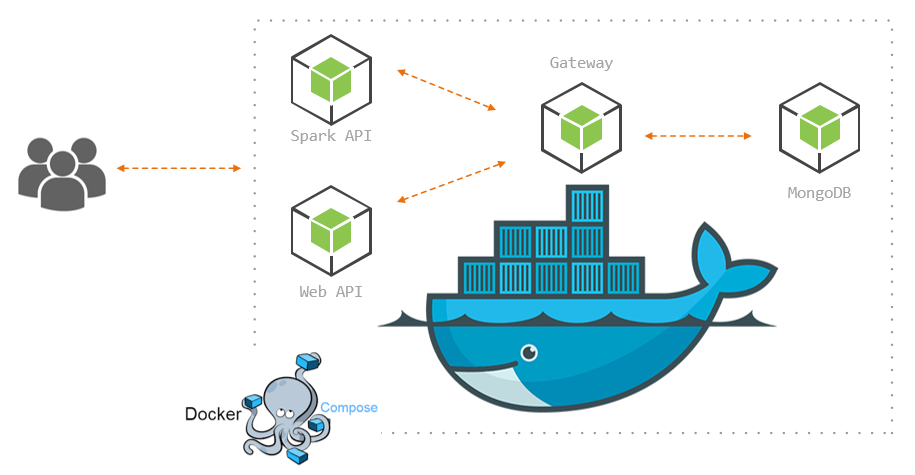
\includegraphics[scale=0.4]{img/docker.png}
	\caption{Docker is platform that can package applications into self contained containers that are able to run in any environment.}
	\label{Literature Review:Docker}
\end{figure}

Docker is a platform for packaging and delivering independent software units in portable and self-sufficient containers that have all the dependencies required for the functionality of their applications. Every container is derived from an image, which essentially is a read-only template. An image provides its container with environmental variables, a command line and a filesystem that can store operating systems, packages, libraries and every other dependency a container needs. The main advantage of encapsulating all the dependencies of a service inside a self-sufficient entity it’s ensuring that the development platform mimics perfectly the target platform. This makes it very easy to continuously integrate and deploy, increases productivity and encourages a frequent feedback loop. With Docker it's possible to package the different types of nodes of an application \cite{docker}. The Front-End and Back-End that implement \ac{MRS} have been packaged into Docker containers.

\newpage
\section{Query optimization through hashing}
A very good algorithm for optimizing comparison between items is locality sensitive hashing (LSH). LSH uses the properties of hashing in order to find similarities between big sized entities \cite{lsh}.
LSH can be used to improve query efficiency through an approximate Membership Query (AMQ) scheme. In such a system, the items are hashed with a similar process as LSH, with the only difference being that instead of hashing the signature into buckets, a Bloom filter is used in the last step to map every item into L bits. All the items that have the same L bits set to 1 are determined to be approximate members of the same data set S. AMQ can be used to produce results within a search engine in O(1) time and has demonstrated better accuracy than LSB-trees and other algorithms than run in at least logarithmic time. However, a good configuration is needed in order to minimize false positives and false negatives \cite{amq}.








